\documentclass[../../main]{subfiles}

\begin{document}
\chapter{準備と前提知識}
\label{chapter:preliminary}

\section{ベクトル空間と行列}

ここでは簡単に(特に有限次元の)ベクトル空間が持つ性質を確かめる.
省略した証明については,たとえば斎藤\cite{saito2020}を参照するとよい.

\subsection{ベクトル空間}

以下,集合\(\numset{K}\)は実数の全体集合\(\numset{R}\)か,複素数の全体集合\(\numset{C}\)であるとする.
\(\numset{K}\)上のベクトル空間とは次のように定義される,加法とスカラー乗法が備わった集合のことである.

\begin{definition}{ベクトル空間}{vector_space}\index{べくとるくうかん@ベクトル空間}
  \(V\)を空でない集合とする.また,任意の\(\vect{x},\vect{y}\in V\),\(s\in\numset{K}\)について,
  和\(\vect{x}+\vect{y}\in V\)とスカラー倍\(s\vect{x}\in V\)が定義されているとする.
  任意の\(\vect{x},\vect{y},\vect{z}\in V\),\(s,t\in\numset{K}\)に対する以下の条件を満たすとき,
  \(V\)は\(\numset{K}\)上の\termdef{ベクトル空間}(vector space)であるという.

  \begin{enumerate}
    \item \((\vect{x}+\vect{y})+\vect{z}=\vect{x}+(\vect{y}+\vect{z})\)
    \item \(\vect{x}+\vect{y}=\vect{y}+\vect{x}\)
    \item ある\(\zvec\in V\)が存在し,任意の\(\vect{v}\in V\)に対して\(\vect{v}+\zvec=\vect{v}\)を満たす.
    \item 各\(\vect{v}\in V\)に対し,\(\vect{w}\in V\)が一意に存在して\(\vect{v}+\vect{w}=\zvec\)を満たす.
    \item \((s+t)\vect{x}=s\vect{x}+t\vect{x}\)
    \item \(s(\vect{x}+\vect{y})=s\vect{x}+s\vect{y}\)
    \item \((st)\vect{x}=s(t\vect{x})\)
    \item \(1\vect{x}=\vect{x}\)
  \end{enumerate}
\end{definition}

しばしば\(V\)の元を\termdef{ベクトル}\index{べくとる@ベクトル}(vector),\(\numset{K}\)の元を\termdef{スカラー}\index{すからー@スカラー}(scalar)と呼ぶ.
また,\cref{definition:vector_space}の\(\zvec\)を\termdef{零ベクトル}\index{ぜろべくとる@零ベクトル}(zero vector),\(\vect{w}\)を\(\vect{v}\)の\termdef{加法逆元}\index{かほうぎゃくげん@加法逆元}(additive inverse)という.
通常,\(\vect{v}\)の加法逆元は\(-\vect{v}\)と表される.

ついで,ベクトル空間にかかわる概念を2つ定義する.

\begin{definition}{線型結合}{linear_combination}\index{せんけいけつごう@線型結合}
  \(V\)を\(\numset{K}\)上のベクトル空間,\(\vect{v}_1,\dots,\vect{v}_n\)を\(V\)の元とする.
  \(c_1\vect{v}_1+\dots+c_n\vect{v}_n\)(\(c_1,\dots,c_n\in\numset{K}\))という形をした\(V\)の元を,
  \(\vect{v}_1,\dots,\vect{v}_n\)の\termdef{線型結合}(linear combination)という.
\end{definition}

\begin{definition}{部分空間}{subspace}\index{ぶぶんくうかん@部分空間}
  \(V\)を\(\numset{K}\)上のベクトル空間,\(W\)を\(V\)の空でない部分集合とする.
  \(W\)が\(V\)の加法とスカラー乗法について\cref{definition:vector_space}の条件をすべて満たすとき,
  \(W\)は\(V\)の\termdef{部分ベクトル空間}(vector subspace),あるいは単に\termdef{部分空間}(subspace)であるという.    
\end{definition}

ある部分集合が部分空間かどうか調べるには,\cref{proposition:subspace_iff}を使うとよい.

\begin{proposition}{}{subspace_iff}
  \(V\)を\(\numset{K}\)上のベクトル空間,\(W\)を\(V\)の空でない部分集合とする.このとき,次の命題は同値である.
  \begin{enumerate}
    \item \(W\)は\(V\)の部分空間である.
    \item 任意の\(s,t\in\numset{K}\),\(\vect{x},\vect{y}\in W\)に対して\(s\vect{x}+t\vect{y}\in W\)である.
  \end{enumerate}
\end{proposition}

\begin{example}
  \(V\)がベクトル空間なら,\(V\)自身と\(\Set{\zvec}\)は\(V\)の部分空間である.
\end{example}

\begin{example}
  集合\(\numset{K}^n=\Set{\trps{\rowvect{s_1 & \cdots & s_n}}\given s_1,\dots,s_n\in\numset{K}}\)は,
  通常の加法とスカラー乗法によって,\(\numset{K}\)上のベクトル空間になる.ただし,\(\trps{\mat{A}}\)\index{T@\(\trps{\mat{A}}\)}は行列\(\mat{A}\)の転置行列を意味する.
\end{example}

また,2つの部分空間\(W_1,W_2\subset V\)があれば,それらを含むより大きな部分空間を作れる.

\begin{definition}{部分空間の和}{sum_of_subspace}\index{わぶぶんくうかんの@和,部分空間の}\index{ぶぶんくうかん@部分空間!わ@和}\indexsymbol{\(V_1+V_2\)}
  \(V\)を\(\numset{K}\)上のベクトル空間,\(W_1,W_2\subset V\)を部分空間とする.
  このとき,集合\(W=\Set{\vect{w}_1+\vect{w}_2\given\text{\(\vect{w}_1\in W_1\),\(\vect{w}_2\in W_2\)}}\)は\(V\)の部分空間になる.
  \(W\)を\(W_1\)と\(W_2\)の\termdef{和}(sum)といい,\(W_1+W_2\)と表記する.
\end{definition}

\(W_1\cap W_2=\Set{\zvec}\)であるとき,\(W_1+W_2\)を\(W_1\)と\(W_2\)の\termdef{直和}\index{ちょくわぶぶんくうかんの@直和,部分空間の}\index{ぶぶんくうかん@部分空間!ちょくわ@直和}(direct sum)という.
直和であることを強調したいときは,和\(W_1+W_2\)を\(W_1\oplus W_2\)\indexsymbol{\(V_1\oplus V_2\)}とも書く.

\subsection{基底}

任意のベクトル\(\vect{x}=\trps{\rowvect{x_1 & \cdots & x_n}}\in\numset{K}^n\)は,第\(i\)成分が\(1\),他の成分が\(0\)のベクトル\(\vect{e}_i\)を用いて\(\vect{x}=x_1\vect{e}_1+\dots+x_n\vect{e}_n\)と表せる.
すなわち,集合\(\basis{S}_n=\Set{\vect{e}_1,\dots,\vect{e}_n}\)は「\(\numset{K}^n\)のすべての元を\(\basis{S}_n\)の元の線型結合で書ける」という性質を持つ.

一般に,ベクトル空間\(V\)の部分集合\(S\)に対して,\(S\)の元の線型結合で書けるベクトルの全体集合を\(S\)が\termdef{生成する部分空間}\index{せいせい@生成!ぶぶんくうかん@部分空間}\index{ぶぶんくうかん@部分空間!せいせいする@生成する\texttwoemdash}(generated subspace)といい,
\(\spannedby S\)\index{span@\(\spannedby S\)}と表記する.この記法を使えば,先述した\(\basis{S}_n\)が持つ性質を「\(\spannedby\basis{S}_n=\numset{K}^n\)が成り立つ」と言い換えられる.

\begin{wrapfigure}[9]{o}{0pt}
  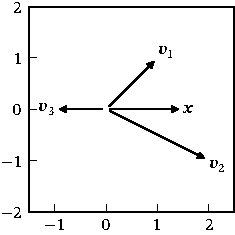
\includegraphics{figures/linear_comb.pdf}
\end{wrapfigure}

\(\spannedby S=\numset{K}^n\)を満たす集合\(S\subset\numset{K}^n\)は,\(\basis{S}_n\)以外にも無数にある.
たとえば\(\numset{K}^n=\numset{R}^2\)のとき,集合\(T=\Set{\vect{v}_1,\vect{v}_2,\vect{v}_3}\)(\(\vect{v}_1=\smallmatrice{1 \\ 1}\),\(\vect{v}_2=\smallmatrice{2 \\ -1}\),\(\vect{v}_3=\smallmatrice{-1 \\ 0}\))が生成する部分空間は\(\numset{R}^2\)である.
しかし,\(\basis{S}_2=\Set{\smallmatrice{1 \\ 0},\smallmatrice{0 \\ 1}}\)の元の線型結合で\(\numset{R}^2\)の元を表す方法はただ1通りであるのに対して,\(T\)はこの性質を持たない.
実際,\(\vect{x}=\smallmatrice{3/2 \\ 0}\)とすると\(\vect{x}=(1/2)\vect{v}_1+(1/2)\vect{v}_2=(-3/2)\vect{v}_3\)である.

\(S\)の元の線型結合で\(\spannedby S\)の元を一意に表せるとき,任意の\(a_i,b_i\in\numset{K}\),\(\vect{v}_i\in S\)について
\[
  \sum_{i=1}^ka_i\vect{v}_i = \sum_{i=1}^kb_i\vect{v}_i
  \implies\matrice{a_1 & \cdots & a_k} = \matrice{b_1 & \cdots & b_k}
\]
が成立する.\(b_1=\dots=b_k=0\)とすると
\begin{equation}
  \label{equation:independence}
  a_1\vect{v}_1+\dots+a_k\vect{v}_k = \zvec
  \implies a_1 = \dots = a_k = 0
\end{equation}
が得られる.

任意の\(a_1,\dots,a_k\in\numset{K}\)に対して\cref{equation:independence}が成立するとき,
\(\vect{v}_1,\dots,\vect{v}_k\)は線型独立であるという.特に,\(V=\spannedby S\)かつ,\(S\)の元からなる有限個のベクトルの組が常に線型独立であるとき,\(S\)は\(V\)の基底であるという.

\begin{definition}{生成系・線型独立・線型従属}{independence}
  \(V\)を\(\numset{K}\)上のベクトル空間,\(S\)を\(V\)の部分集合とする.また,\(\vect{v}_1,\dots,\vect{v}_k\)を\(V\)の元とする.
  \begin{enumerate}
    \item \(V=\spannedby S\)であるとき,\(S\)を\(V\)の\termdef{生成系}(generating set)という.
    \item \(\sum_{i=1}^kc_i\vect{v}_i=\zvec\)を満たす\(c_1,\dots,c_k\in\numset{K}\)の組が\(c_1=\dots=c_k=0\)しかないとき,\(\vect{v}_1,\dots,\vect{v}_k\)は\termdef{線型独立}\index{せんけいどくりつ@線型独立}(linearly independent)であるという.
    \item \(\vect{v}_1,\dots,\vect{v}_k\)が線型独立でないとき,\(\vect{v}_1,\dots,\vect{v}_k\)は\termdef{線型従属}\index{せんけいじゅうぞく@線型従属}(linearly dependent)であるという.
  \end{enumerate}
\end{definition}

\begin{definition}{基底}{basis}
  \(V\)を\(\numset{K}\)上のベクトル空間,\(\basis{B}\)を\(V\)の部分集合とする.
  \(\basis{B}\)が\(V\)の生成系かつ,\(\basis{B}\)に属する有限個のベクトル\(\vect{v}_1,\dots,\vect{v}_k\)が常に線型独立であるとき,\(\basis{B}\)は\(V\)の\termdef{基底}\index{きてい@基底}(basis)であるという.
\end{definition}

\begin{example}[標準基底]
  \(\basis{S}_n\)は\(\numset{K}^n\)の基底である.\(\basis{S}_n\)を\(\numset{K}^n\)の\termdef{標準基底}\index{ひょうじゅんきてい@標準基底}(standard basis)という.
\end{example}

さきほどの議論によれば,\(S\)の元の線型結合で\(\spannedby S\)の元を一意に表せるとき,任意の\(a_1,\dots,a_k\in\numset{K}\)について\cref{equation:independence}が成立する.
すなわち,\(S\)は\(\spannedby S\)の基底である.この逆も成り立つので,次の命題が成立する.

\begin{proposition}{}{span_and_uniqueness}
  \(V\)を\(\numset{K}\)上のベクトル空間,\(S\)を\(V\)の部分集合とする.このとき,次の命題は同値である.
  \begin{enumerate}
    \item \(S\)の元の線型結合で\(\spannedby S\)の元を一意に表せる.
    \item \(S\)は\(\spannedby S\)の基底である.
  \end{enumerate}
\end{proposition}

\(V\)の基底で有限集合のものがあるとき,\(V\)は\termdef{有限次元}\index{ゆうげんじげん@有限次元}(finite-dimensional)であるという.
\(V\)が有限次元なら,\(V\)の基底はすべて有限集合で,その元の個数は等しい.
すなわち,元の個数\(\sizeof{\basis{B}}\)は基底\(\basis{B}\)のとりかたによらず定まる.
\(\sizeof{\basis{B}}\)を\(V\)の\termdef{次元}\index{じげん@次元}(dimension)といい,\(\dim V\)\index{dim@\(\dim V\)}と表記する
\footnote{任意のベクトル空間は基底を持つ(雪江\cite{yukie2019}に証明がある)が,有限集合とは限らない.}.

基底に関連して,次の命題が成り立つ.

\begin{proposition}{}{basis_and_matrix}
  \(\vect{v}_1,\dots,\vect{v}_n\in\numset{K}^n\)とする.このとき,次の命題は同値である.
  \begin{enumerate}
    \item 集合\(\Set{\vect{v}_1,\dots,\vect{v}_n}\)は\(\numset{K}^n\)の基底である.
    \item 行列\(\rowvect{\vect{v}_1 & \cdots & \vect{v}_n}\)は正則である.
  \end{enumerate}
\end{proposition}

\begin{proposition}{基底の延長}{basis_extension}
  \(V\)を\(\numset{K}\)上の\(n\)次元ベクトル空間とする.\(k<n\)個のベクトル\(\vect{v}_1,\dots,\vect{v}_k\in V\)が線型独立なら,
  集合\(\Set{\vect{v}_1,\dots,\vect{v}_k,\vect{v}_{k+1},\dots,\vect{v}_n}\)が\(V\)の基底になる\(\vect{v}_{k+1},\dots,\vect{v}_n\in V\)が存在する.
\end{proposition}

\subsection{内積}

\(\numset{R}^3\)において,ベクトルの長さとなす角はドット積\((x_1,x_2,x_3)\cdot(y_1,y_2,y_3)=\sum_{i=1}^3x_iy_i\)から計算できた.
次の定義はドット積を抽象化したものである.

\begin{definition}{内積}{inner_product}\index{ないせき@内積}\indexsymbol{\(\innerp{\holder}{\holder}\)}
  \(V\)を\(\numset{K}\)上のベクトル空間とする.\(\innerp{\holder}{\holder}\)が\(V\)の\termdef{内積}(inner product)であるとは,
  任意の\(\lambda\in\numset{K}\),\(\vect{x},\vect{y},\vect{z}\in V\)に対し,\(\innerp{\holder}{\holder}\)が以下の条件を満たすことをいう.
  \begin{enumerate}
    \item \(\innerp{\vect{x}}{\vect{y}}=\conj*{\innerp{\vect{y}}{\vect{x}}}\in\numset{K}\)
    \item \(\innerp{\lambda\vect{x}+\vect{y}}{\vect{z}}=\lambda\innerp{\vect{x}}{\vect{z}}+\innerp{\vect{y}}{\vect{z}}\)
    \item \(\innerp{\vect{x}}{\vect{x}}\geq 0\),\([\innerp{\vect{x}}{\vect{x}}=0\iff\vect{x}=\zvec]\)
  \end{enumerate}
\end{definition}

内積が備わっているベクトル空間のことを\termdef{内積空間}\index{ないせきくうかん@内積空間}(inner product space)という.
また,\(\innerp{\vect{v}}{\vect{w}}=0\)であるときベクトル\(\vect{v}\)と\(\vect{w}\)は\termdef{直交}\index{ちょっこう@直交}するという.

\begin{example}[標準内積]
  \(\innerp{\vect{v}_1}{\vect{v}_2}=\trps{\vect{v}_1}\conj{\vect{v}}_2\)(\(\vect{v}_1,\vect{v}_2\in\numset{K}^n\))とすると,
  \(\innerp{\holder}{\holder}\)は\(\numset{K}^n\)の内積になる.\(\innerp{\holder}{\holder}\)を\(\numset{K}^n\)の\termdef{標準内積}\index{ひょうじゅんないせき@標準内積}という.
\end{example}

\begin{definition}{正規直交系,正規直交基底}{onb}\index{せいきちょっこうけい@正規直交系}\index{せいきちょっこうきてい@正規直交基底}\index{ONS|see{正規直交系}}\index{ONB|see{正規直交基底}}
  \(V\)を内積空間,\(\basis{B}\)を\(V\)の空でない部分集合とする.\(\basis{B}\)の相異なる2元が常に直交し,すべての\(\vect{e}\in\basis{B}\)が\(\innerp{\vect{e}}{\vect{e}}=1\)を満たすとき,
  \(\basis{B}\)は\termdef{正規直交系}(orthonormal system; ONS)であるという.また,正規直交系である基底を\termdef{正規直交基底}(orthonormal basis; ONB)という.
\end{definition}

\(\basis{B}\)が正規直交系なら,有限個の\(\basis{B}\)の元からなる組はすべて線型独立である.
よって,\(\basis{B}\)が基底であることを見るには\(V=\spannedby\basis{B}\)だけ確かめればよい.

また,内積空間に属する線型独立なベクトルの組があれば,それらから正規直交系を作れる.

\begin{proposition}{グラム・シュミットの直交化法}{gram_schmidt}\index{ぐらむしゅみっとのちょっこうかほう@グラム・シュミットの直交化法}
  \(V\)を内積空間とする.\(\vect{v}_1,\dots,\vect{v}_n\in V\)が線型独立なら
  \[
    \vect{u}_1 = \vect{v}_1,
    \quad\vect{u}_i = \vect{v}_i-\sum_{j=1}^{n-1}\frac{\innerp{\vect{v}_i}{\vect{u}_j}}{\innerp{\vect{u}_j}{\vect{u}_j}}\vect{u}_j\quad(i=2,\dots,n)
  \]
  で\(\vect{u}_i\)を定義すると,集合\(\Set{\vect{u}_i/\sqrt{\innerp{\vect{u}_i}{\vect{u}_i}}\given i=1,\dots,n}\)は\(V\)の正規直交系になる.
  正規直交系を作るこの方法を\termdef{グラム・シュミットの直交化法}(Gram–Schmidt orthogonalization)という.
\end{proposition}

\subsection{線型写像と表現行列}
\label{subsection:representation_matrix}

\(V\)は有限次元とする.\cref{proposition:span_and_uniqueness}によれば,\(V\)の基底\(\basis{B}=\Set{\vect{v}_1,\dots,\vect{v}_m}\)を選ぶと,任意の\(\vect{x}\in V\)を
\begin{equation}
  \label{equation:basis_comb}
  \vect{x} = c_1\vect{v}_1+\dots+c_m\vect{v}_m\quad(c_1,\dots,c_m\in\numset{K})
\end{equation}
の形で一意に表せる.言い換えれば,\(V\)の各元\(\vect{x}\)に\cref{equation:basis_comb}の\(\trps{\rowvect{c_1 & \cdots & c_m}}\)を割り当てる写像\(\phi\colon V\to\numset{K}^m\)を定義でき,それは単射である
\index{たんしゃ@単射}\footnote{写像\(f\)の定義域に属する任意の\(x,y\)について,命題「\(f(x)=f(y)\implies x=y\)」が成立するとき,\(f\)は\termdef{単射}(injection)であるという.}.この写像\(\phi\)は,次に定義する「線型写像」の1例である.

\begin{definition}{線型写像}{linear_mapping}\index{せんけいしゃぞう@線型写像}
  \(V\)と\(W\)を\(\numset{K}\)上のベクトル空間とする.写像\(f\colon V\to W\)が以下の条件を満たすとき,\(f\)は\termdef{線型写像}(linear mapping)であるという.
  \begin{enumerate}
    \item 任意の\(\vect{x},\vect{y}\in V\)に対して\(f(\vect{x}+\vect{y})=f(\vect{x})+f(\vect{y})\)である.
    \item 任意の\(c\in\numset{K}\),\(\vect{x}\in V\)に対して\(f(c\vect{x})=cf(\vect{x})\)である.
  \end{enumerate}
\end{definition}

\(W\)を\(\numset{K}\)上の有限次元ベクトル空間とする.\(W\)の基底\(\basis{B}'=\Set{\vect{w}_1,\dots,\vect{w}_n}\)(\(n=\dim W\))をとると,\(\phi\)と同様
\[
  \vect{y} = d_1\vect{w}_1+\dots+d_n\vect{w}_n
  \iff\psi(\vect{y}) = \trps{\matrice{d_1 & \cdots & d_n}}
\]
を満たす線型写像\(\psi\colon W\to\numset{K}^n\)が定義できる.

\(\phi\)と\(\psi\)を利用すると,\(V\)から\(W\)への任意の線型写像\(f\)を,対応する行列によって表現できる.
\(\vect{x}\in V\)を任意にとる.\(\phi(\vect{x})=\trps{\rowvect{c_1 & \cdots & c_m}}\)とおくと
\begin{gather*}
  f(\vect{x}) = f\pqty*{\sum_{i=1}^mc_i\vect{v}_i} = \sum_{i=1}^mc_if(\vect{v}_i), \\
  \psi(f(\vect{x})) = \sum_{i=1}^mc_i\psi(f(\vect{v}_i))
  = \matrice{\psi(f(\vect{v}_1)) & \cdots & \psi(f(\vect{v}_m))}\matrice*{c_1 \\ \vdots \\ c_m}
\end{gather*}
であるから,\(\mat{A}=\rowvect{\psi(f(\vect{v}_1)) & \cdots & \psi(f(\vect{v}_m))}\),\(T(\vect{x})=\mat{A}\vect{x}\)とおくと
\begin{equation}
  \label{equation:representation_matrix}
  \psi(f(\vect{x})) = T(\phi(\vect{x}))
\end{equation}
が成り立つ.

\begin{wrapfigure}[5]{o}{0pt}
  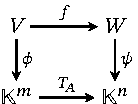
\includegraphics{figures/commute.pdf}
\end{wrapfigure}

ここまでの議論をまとめると,次のようになる.\(V\)の基底\(\basis{B}\)と,\(W\)の基底\(\basis{B}'\)をとるごとに,
\(n\times m\)行列\(\mat{A}=\rowvect{\psi(f(\vect{v}_1)) & \cdots & \psi(f(\vect{v}_m))}\)を定義でき,
\(\mat{A}\)は\cref{equation:representation_matrix}を満たす.
この\(\mat{A}\)を,基底\(\basis{B}\)と\(\basis{B}'\)に関する\(f\)の\termdef{表現行列}\index{ひょうげんぎょうれつ@表現行列}\index{ぎょうれつ@行列!ひょうげん@表現\texttwoemdash}(representation matrix)という.

なお,\(\basis{B}\)の元を並べる順序に応じて,\cref{equation:basis_comb}の\(c_1,\dots,c_n\)の順序も変化するので,
\(\phi\)は\(\basis{B}\)に対して一意ではない.\(\phi\)は\(\basis{B}\)の元を並べる順序を決めて初めて定まる.
本書では,\(\basis{B}=\Set{\vect{v}_1,\dots,\vect{v}_n}\)のような書き方をした場合,\(\basis{B}\)の元を\(\vect{v}_1,\vect{v}_2,\dotsc\)の順に並べると決めておく.

\begin{example}[形式的な微分]
  次数が\(n\)未満の1変数多項式全体\(V_n=\Set{c_0+c_1x+\dots+c_{n-1}x^{n-1}\given c_0,\dots,c_{n-1}\in\numset{R}}\)は,\(\numset{R}\)上の\(n\)次元ベクトル空間である.
  また,写像\(D\colon V_4\to V_3\)を\(D(c_0+c_1x+c_2x^2)=c_1+2c_2x\)で定義すると,これは線型写像になる.
  \(V_n\)の基底として\(\basis{B}_n=\Set{1,x,\dots,x^{n-1}}\)をとったとき,基底\(\basis{B}_4\)と\(\basis{B}_3\)に関する\(D\)の表現行列は\(\smallmatrice{0 & 1 & 0 \\ 0 & 0 & 2}\)である.
\end{example}

\subsection{核と像}

線型写像に付随して,重要なベクトル空間が2つ定まる.

\begin{definition}{核,像}{nul_img}\index{かく@核}\index{ぞう@像}\index{ker@\(\nul f\)}\index{im@\(\img f\)}
  \(f\colon V\to W\)を線型写像とする.
  \begin{enumerate}
    \item \(V\)の部分空間\(\inv{f}{\Set{\vect{0}}}\)を\(f\)の\termdef{核}(kernel)といい,\(\nul f\)と表す.
    \item \(W\)の部分空間\(\ran{f}{V}\)を\(f\)の\termdef{像}(image)といい,\(\img f\)と表す.
  \end{enumerate}
\end{definition}

\begin{note}
  写像\(f\colon X\to Y\)と集合\(A\subset X\),\(B\subset Y\)に関して\(\ran{f}{A}=\Set{f(x)\given x\in A}\)\indexsymbol{\(\ran{f}{S}\)},
  \(\inv{f}{B}=\Set{x\in X\given f(x)\in B}\)\indexsymbol{\(\inv{f}{S}\)}である.\(\ran{f}{A}\)を\(f\)による\(A\)の\termdef{像}\index{ぞう@像}(image),
  \(\inv{f}{B}\)を\(f\)による\(B\)の\termdef{逆像}\index{ぎゃくぞう@逆像}(inverse image)という.
\end{note}

\begin{proposition}{}{nul_and_uniqueness}
  \(f\colon V\to W\)を線型写像とする.このとき,\(f\)が単射であることと,\(\nul f=\Set{\zvec}\)が成立することは同値である.
\end{proposition}

\begin{proof}
  \(f(\zvec)=f(\zvec+\zvec)=f(\zvec)+f(\zvec)\)なので,\(f(\zvec)=\zvec\)である.よって,\(f\)が単射なら\(\nul f=\Set{\zvec}\)である.
  また,\(\vect{v}_1,\vect{v}_2\in V\)が\(f(\vect{v}_1)=f(\vect{v}_2)\)を満たせば\(f(\vect{v}_1-\vect{v}_2)=f(\vect{v}_1)-f(\vect{v}_2)=\zvec\)である.
  よって,\(\nul f=\Set{\zvec}\)なら\(\vect{v}_1-\vect{v}_2=\zvec\)である.すなわち,\(\nul f=\Set{\zvec}\)なら\(f\)は単射である.
\end{proof}

\subsection{固有値と固有空間}

対角化に向けて,固有値に関連する事項を整理する.

\begin{definition}{固有値,固有ベクトル}{eigenvalue}\index{こゆうち@固有値}\index{こゆうべくとる@固有ベクトル}
  \(\mat{A}\)を\(n\)次正方行列とする.
  複素数\(\lambda\)と\(\zvec\)でないベクトル\(\vect{x}\in\numset{C}^n\)が式\(\mat{A}\vect{x}=\lambda\vect{x}\)を満たすとき,
  \(\lambda\)を\(\mat{A}\)の\termdef{固有値}(eigenvalue)という.
  また,\(\vect{x}\)を\(\mat{A}\)の(固有値\(\lambda\)に属する)\termdef{固有ベクトル}(eigenvector)という.
\end{definition}

\begin{definition}{固有空間}{eigenspace}\index{こゆうくうかん@固有空間}\index{e@\(E_\lambda(\mat{A})\)}
  \cref{definition:eigenvalue}の\(\mat{A}\),\(\lambda\)について,集合\(E_\lambda(\mat{A})=\Set{\vect{x}\in\numset{C}^n\given\mat{A}\vect{x}=\lambda\vect{x}}\)は\(\numset{C}^n\)の部分空間になる.
  部分空間\(E_\lambda(\mat{A})\)を,\(\mat{A}\)の(固有値\(\lambda\)に属する)\termdef{固有空間}(eigenspace)という.
\end{definition}

\begin{example}
  \(\vect{x}_1=\trps{\rowvect{1+\iuni & 2}}\),\(\vect{x}_2=\trps{\rowvect{1-\iuni & 2}}\)は\(\mat{A}=\smallmatrice{1 & -1 \\ 2 & -1}\)の固有ベクトルである.
  実際\(\mat{A}\vect{x}_1=\iuni\vect{x}_1\),\(\mat{A}\vect{x}_2=-\iuni\vect{x}_2\)である.
\end{example}

以下,\(\mat{A}\)を任意の\(n\)次正方行列,\(\spec\mat{A}\)\index{spec@\(\spec\mat{A}\)}を\(\mat{A}\)の固有値の全体集合とする.

\(n\)次多項式\(P(\lambda)=\det(\lambda\imat-\mat{A})\)を\(\mat{A}\)の\termdef{固有多項式}\index{こゆうたこうしき@固有多項式}(characteristic polynomial)という.
\cref{proposition:characteristic_polynomial}から,\(\mat{A}\)の固有値を求めることは,方程式\(P(\lambda)=0\)を解くことと同義である.

\begin{proposition}{}{characteristic_polynomial}
  \(\spec\mat{A}=\Set{\lambda\in\numset{C}\given\det(\lambda\imat-\mat{A})=0}\)である.
\end{proposition}

また,固有空間は次の性質を持つ.

\begin{proposition}{}{eigenspaces_disjointness}
  \(\lambda_1,\lambda_2\in\spec\mat{A}\),\(\lambda_1\neq\lambda_2\)ならば\(E_{\lambda_1}(\mat{A})\cap E_{\lambda_2}(\mat{A})=\Set{\zvec}\)である.
\end{proposition}

\begin{proof}
  \(\vect{x}\in E_{\lambda_1}(\mat{A})\cap E_{\lambda_2}(\mat{A})\)とすると,\(\mat{A}\vect{x}=\lambda_1\vect{x}=\lambda_2\vect{x}\)より\((\lambda_1-\lambda_2)\vect{x}=\zvec\)であり,
  \(\lambda_1\neq\lambda_2\)なので\(\vect{x}=\zvec\)である.よって\(E_{\lambda_1}(\mat{A})\cap E_{\lambda_2}(\mat{A})\)は\(\zvec\)以外に元を持たない.
\end{proof}

\subsection{対角化}

適当な\(n\)次正則行列\(\mat{P}\),対角行列\(\mat{\Lambda}\)の組を見つけて,\(n\)次正方行列\(\mat{A}\)を\(\mat{A}=\mat{P}\mat{\Lambda}\mat{P}^{-1}\)の形で書くことを
\(\mat{A}\)の\termdef{対角化}\index{たいかくか@対角化}(diagonalization)という.\(\mat{A}\)が対角化可能である必要十分条件は,次の\cref{proposition:diagonalization}で与えられる.

\begin{proposition}{}{diagonalization}
  \(\mat{A}\)に関する以下の条件は同値である.
  \begin{enumerate}
    \item \(\mat{A}\)の固有ベクトルのみからなる\(\numset{K}^n\)の基底が存在する.
    \item \(\numset{K}^n=\bigoplus_{\lambda\in\spec\mat{A}}E_\lambda(\mat{A})\)が成立する.
    \item \(n\)次正則行列\(\mat{P}\),対角行列\(\mat{\Lambda}\)が存在して\(\mat{A}=\mat{P}\mat{\Lambda}\mat{P}^{-1}\)を満たす.
  \end{enumerate}
\end{proposition}

以下,対角行列\(\smallmatrice{a_1 & & \\ & \ddots & \\ & & a_n}\)を\(\diag(a_1,\dots,a_n)\)\index{diag@\(\diag(a_1,\dots,a_n)\)}と略記する.

\begin{proof}
  1と3の同値性のみ示す.\(\mat{A}\)の固有ベクトルのみからなる\(\numset{K}^n\)の基底\(\Set{\vect{v}_1,\dots,\vect{v}_n}\)があるとき,\(\mat{A}\)は対角化できることを示す.
  \(\mat{P}=\rowvect{\vect{v}_1 & \cdots & \vect{v}_n}\)とおく.このとき,各\(\vect{v}_i\)に対応する固有値を\(\lambda_i\)とおくと
  \(\mat{A}\mat{P}=\rowvect{\mat{A}\vect{v}_1 & \cdots & \mat{A}\vect{v}_n}=\rowvect{\lambda_1\vect{v}_1 & \cdots & \lambda_n\vect{v}_n}\)
  だから,\(\mat{\Lambda}=\diag(\lambda_1,\dots,\lambda_n)\)とおくと\(\mat{A}\mat{P}=\mat{P}\mat{\Lambda}\),\(\mat{A}=\mat{P}\mat{\Lambda}\mat{P}^{-1}\)となる.
  ただし,\(\mat{P}\)の逆行列が存在することは\cref{proposition:basis_and_matrix}による.

  逆に,\(\mat{A}=\mat{P}\mat{\Lambda}\mat{P}^{-1}\)を満たす\(n\)次正則行列\(\mat{P}\),対角行列\(\mat{\Lambda}\)が存在したとする.
  \(\mat{P}=\rowvect{\vect{v}_1 & \cdots & \vect{v}_n}\),\(\mat{\Lambda}=\diag(\lambda_1,\dots,\lambda_n)\)とおく.
  すると\(\rowvect{\mat{A}\vect{v}_1 & \cdots & \mat{A}\vect{v}_n}=\mat{A}\mat{P}=\mat{P}\mat{\Lambda}=\rowvect{\lambda_1\vect{v}_1 & \cdots & \lambda_n\vect{v}_n}\)なので,
  各\(\lambda_i\),\(\vect{v}_i\)は\(\mat{A}\vect{v}_i=\lambda_i\vect{v}_i\)を満たす.
  また,\(\mat{P}\)は正則だから\(\vect{v}_i\neq\zvec\)である.よって\cref{proposition:basis_and_matrix}より,集合\(\Set{\vect{v}_1,\dots,\vect{v}_n}\)は\(\mat{A}\)の固有ベクトルからなる\(\numset{K}^n\)の基底である.
\end{proof}

\section{微分積分学}

ここでは\(\varepsilon\mathhyphen N\)論法による極限の定義を既知として,実数の性質からしたがう事実をいくつか挙げる.
なお,紙幅の都合で証明はほぼ省略した.興味があれば杉浦\cite{sugiura2018}を参照するとよい.

\subsection{上限と下限}

\begin{definition}{上界,下界}{}\index{じょうかい@上界}\index{かかい@下界}
  \(X\)を\(\numset{R}\)の部分集合とする.
  \begin{enumerate}
    \item 実数\(a\)が\(X\)の\termdef{上界}(upper bound)であるとは,任意の\(x\in X\)に対して\(x\leq a\)が成立することをいう.
    \item 実数\(b\)が\(X\)の\termdef{\ltjruby{下界}{かかい}}(lower bound)であるとは,任意の\(x\in X\)に対して\(x\geq b\)が成立することをいう.
  \end{enumerate}
\end{definition}

\(X\)の上界が存在するとき,\(X\)は\termdef{上に有界}であるという.同様に,\(X\)の下界が存在するとき,\(X\)は\termdef{下に有界}であるという.
\(X\)が上にも下にも有界\texttwoemdash つまり集合\(\Set{\abs{x}\given x\in X}\)が上に有界\texttwoemdash なときは,単に\termdef{有界}\index{ゆうかい@有界}であるという.

\begin{definition}{上限,下限}{}\index{じょうげん@上限}\index{かげん@下限}\index{sup@\(\sup S\)}\index{inf@\(\inf S\)}
  \(X\)を\(\numset{R}\)の空でない部分集合とする.
  \begin{enumerate}
    \item \(X\)が上に有界であれば,上界の全体集合は最小元\(m\)を持つ.\(m\)を\(X\)の\termdef{上限}(supremum)といい,\(\sup X\)と書く.
    \item \(X\)が下に有界であれば,下界の全体集合は最大元\(M\)を持つ.\(M\)を\(X\)の\termdef{下限}(infimum)といい,\(\inf X\)と書く.
  \end{enumerate}
\end{definition}

便宜上,\(X\)が上に有界でないときは\(\sup X=+\infty\),\(X\)が下に有界でないときは\(\inf X=-\infty\)と決めておく.
上限と下限を用いて議論するときは,次の\cref{proposition:sup_inf_and_eps}が便利である.

\begin{proposition}{}{sup_inf_and_eps}
  \(X\)を\(\numset{R}\)の部分集合とする.このとき,実数\(s\)に関する以下の条件は同値であり,同様のことが\(\inf X\)についても成り立つ.
  \begin{enumerate}
    \item \(s=\sup X\)である.
    \item 任意の\(\varepsilon>0\)に対し,\(x\in X\)が存在して\(x+\varepsilon>s\)を満たす.
  \end{enumerate}
\end{proposition}

\subsection{数列の極限}

数列の各項からなる集合が有界であるとき,その数列は有界であるという.

\begin{proposition}{}{monotone_converge}
  実数列\(\seq{a_n}_{n\in\numset{N}}\)は上に有界とする.このとき,\(a_1\leq a_2\leq\dotsb\)なら\(\seq{a_n}_{n\in\numset{N}}\)は収束する.
\end{proposition}

\begin{proof}
  \(\alpha=\sup S\)とする.このとき\(a_n\to\alpha\)(\(n\to\infty\))であることを示す.
  任意に\(\varepsilon>0\)をとる.\cref{proposition:sup_inf_and_eps}より,\(x+\varepsilon>\alpha\)となる\(x\in S\)がある.
  \(x=a_N\)を満たす\(N\)について,\(n\geq N\)なら\(a_N\leq a_n\leq\alpha\),\(\abs{a_n-\alpha}=\alpha-a_n\leq\alpha-a_N<\varepsilon\)である.
  よって\(a_n\to\alpha\)(\(n\to\infty\))である.
\end{proof}

\begin{definition}{上極限,下極限}{}\index{じょうきょくげん@上極限}\index{かきょくげん@下極限}\index{limsup@\(\limsup\)}\index{liminf@\(\liminf\)}
  実数列\(\seq{a_n}_{n\in\numset{N}}\)に対して,\(\limsup_{n\to\infty}a_n\)と\(\liminf_{n\to\infty}a_n\)を
  \begin{gather*}
    \limsup_{n\to\infty}a_n = \lim_{n\to\infty}\sup\Set{a_n,a_{n+1},\dotsc}, \\
    \liminf_{n\to\infty}a_n = \lim_{n\to\infty}\inf\Set{a_n,a_{n+1},\dotsc}
  \end{gather*}
  で定義する.\(\limsup_{n\to\infty}a_n\)を数列\(\seq{a_n}_{n\in\numset{N}}\)の\termdef{上極限}(limit superior),
  \(\liminf_{n\to\infty}a_n\)を数列\(\seq{a_n}_{n\in\numset{N}}\)の\termdef{下極限}(limit inferior)という.
\end{definition}

\cref{proposition:monotone_converge}より\(\limsup_{n\to\infty}a_n<+\infty\iff\sup\Set{a_1,a_2,\dotsc}<+\infty\)であり,
同様のことが\(\liminf_{n\to\infty}a_n\)についても成り立つ.また,次のことが知られている.

\begin{proposition}{}{}
  \(\seq{a_n}_{n\in\numset{N}}\)を実数列とする.このとき,実数\(\alpha\)に関する以下の条件は同値である.
  \begin{enumerate}
    \item \(a_n\to\alpha\)(\(n\to\infty\))である.
    \item \(\liminf_{n\to\infty}a_n=\limsup_{n\to\infty}a_n=\alpha\)である.
  \end{enumerate}
\end{proposition}

\cref{xr-chapter:hilbert_space}以降では,望ましい性質を持つ収束列を定義して,その極限によって命題を示すことが多くなる.
極限値が予想できる場合を除き,数列が収束することを示すには,それがコーシー列であることを示すのがよい.

\begin{definition}{コーシー列}{real_cauchy_sequence}\index{こーしーれつ@コーシー列}
  \(\seq{x_n}_{n\in\numset{N}}\)を実数列とする.\(\seq{x_n}_{n\in\numset{N}}\)が\termdef{コーシー列}(Cauchy sequence)であるとは,
  任意の\(\varepsilon>0\)に対し,\(N\in\numset{N}\)が存在して\(m,n>N\implies\abs{x_m-x_n}<\varepsilon\)を満たすことをいう.このことを次のように表す.
  \[
    \abs{x_m-x_n} \to 0\quad(m,n\to\infty),
    \quad\lim_{m,n\to\infty}\abs{x_m-x_n} = 0
  \]
\end{definition}

実数列について,数列がコーシー列であることと収束列であることは同値である.ただし,コーシー列であることは極限値を使わずに確かめられる.

\begin{example}
  \(a_n=\sum_{i=0}^n(-1)^i/(i!)\)とする.このとき,\(m>n\geq N\)なら
  \[
    \abs{a_m-a_n} \leq \sum_{i=n+1}^m\frac{1}{i!}
    \leq \sum_{i=n+1}^m\frac{1}{i(i-1)}
    = \sum_{i=n+1}^m\pqty*{\frac{1}{i-1}-\frac{1}{i}}
    = \frac{1}{n}-\frac{1}{m}
  \]
  であり,\(1/n-1/m\leq 1/N\to 0\)(\(N\to\infty\))だから\(\seq{a_n}_{n\in\numset{N}}\)はコーシー列である.
  よって,級数\(\sum(-1)^n/(n!)\)は収束する(よく知られているように,この値は\(1/\napr\)である).
\end{example}

\end{document}
